%Tendo encontrado o modelo cinemático, representado por $T_7^0$, é importante realizar sua validação. Isso pode ser feito através de análise dimensional ou por simulação computacional. No primeiro caso o modelo é aplicado à duas situações de conjuntos de valores das variáveis de juntas, sendo gerado a pose do \textit{end-effector}. Com isto, é comparado os resultados da matriz de transformação com o comportamento esperado.

%Para verificar a coerência do modelo obtido com o robô real foram escolhidas as condições de posição inicial de todos os ângulos em zero (conhecida como \textit{home}) e uma segunda condição para os ângulos $\theta_4 = -\pi/2$ e $\theta_5 = \pi/3$, mantendo os demais ângulos em zero. Assim foram obtidas as matrizes $T_\mathrm{home}$ e $T_\mathrm{escolhido}$, respectivamente.


Tendo encontrado o modelo cinemático, representado por $T_7^0$, é importante realizar sua validação. Isto é, verificar a coerência entre a representação matemática e o robô real. Isso pode ser feito através de análise dimensional ou por simulação computacional. No primeiro caso, é aplicado ao modelo um conjunto de valores de entrada, ou seja, são aplicados na matriz $T_7^0$ um conjunto de valores para os ângulos das juntas. Assim, obtém-se uma matriz que representa a pose do \textit{end-effector} em relação ao \textit{frame} 0 que deve corresponder ao diagrama de arames desenhado para a entrada de dados aplicada ao modelo. É recomendado que esse procedimento seja feito para duas entradas diferentes.

Nesse trabalho aplicou-se um conjunto de ângulos que representam a posição \textit{home}, $\theta_i=0$ para $i= 1, ... , 7$ e outro conjunto para uma posição escolhida dada por $\theta_1=\theta_2=\theta_3=\theta_6=\theta_7=0$, $\theta_4 = -\pi/2$ e $\theta_5 = \pi/3$. Assim, aplicando os ângulos das juntas nas equações apresentadas no Apêndice \ref{apend:MatrizT}, foram obtidas as matrizes
\begin{align}
T_\mathrm{home}
    &=
    \left[ 
    \begin{array}{rrr;{2pt/2pt}c}
        1 & 0 &  0 & 0 \\
        0 & 1 & 0 & 0 \\
        0 & 0 & 1 & 1270 \\
        \hdashline[2pt/2pt]
        0 & 0 & 0 & 1
    \end{array}
    \right],
    \label{eq:Thome} \\
T_\mathrm{escolhido}
    &=
    \left[ 
    \begin{array}{rrr;{2pt/2pt}c}
        0 & 0 & 1 & 490 \\
        \frac{\sqrt{3}}{2} & \frac{1}{2} &  0 & 0 \\
        -\frac{1}{2} & \frac{\sqrt{3}}{2} & 0 & 780 \\
        \hdashline[2pt/2pt]
        0 & 0 & 0 & 1
    \end{array}
    \right].
    \label{eq:Tescolhido}
\end{align}

A matriz $T_\mathrm{home}$ confirma as duas características da pose do robô em \textit{home}. A primeira é a translação que se concentra apenas no eixo $z$ cujo valor é a soma das extensões de todos os links. A segunda característica se refere à rotação, a qual percebe-se ser de valor zero nos três eixos devido à matriz de rotação estar expressa como uma matriz identidade. A representação em diagrama de arames desta condição confirma as características supracitadas e pode ser visto na FIG. \ref{diagramahome}.
\begin{figure}[h]
    \centering
    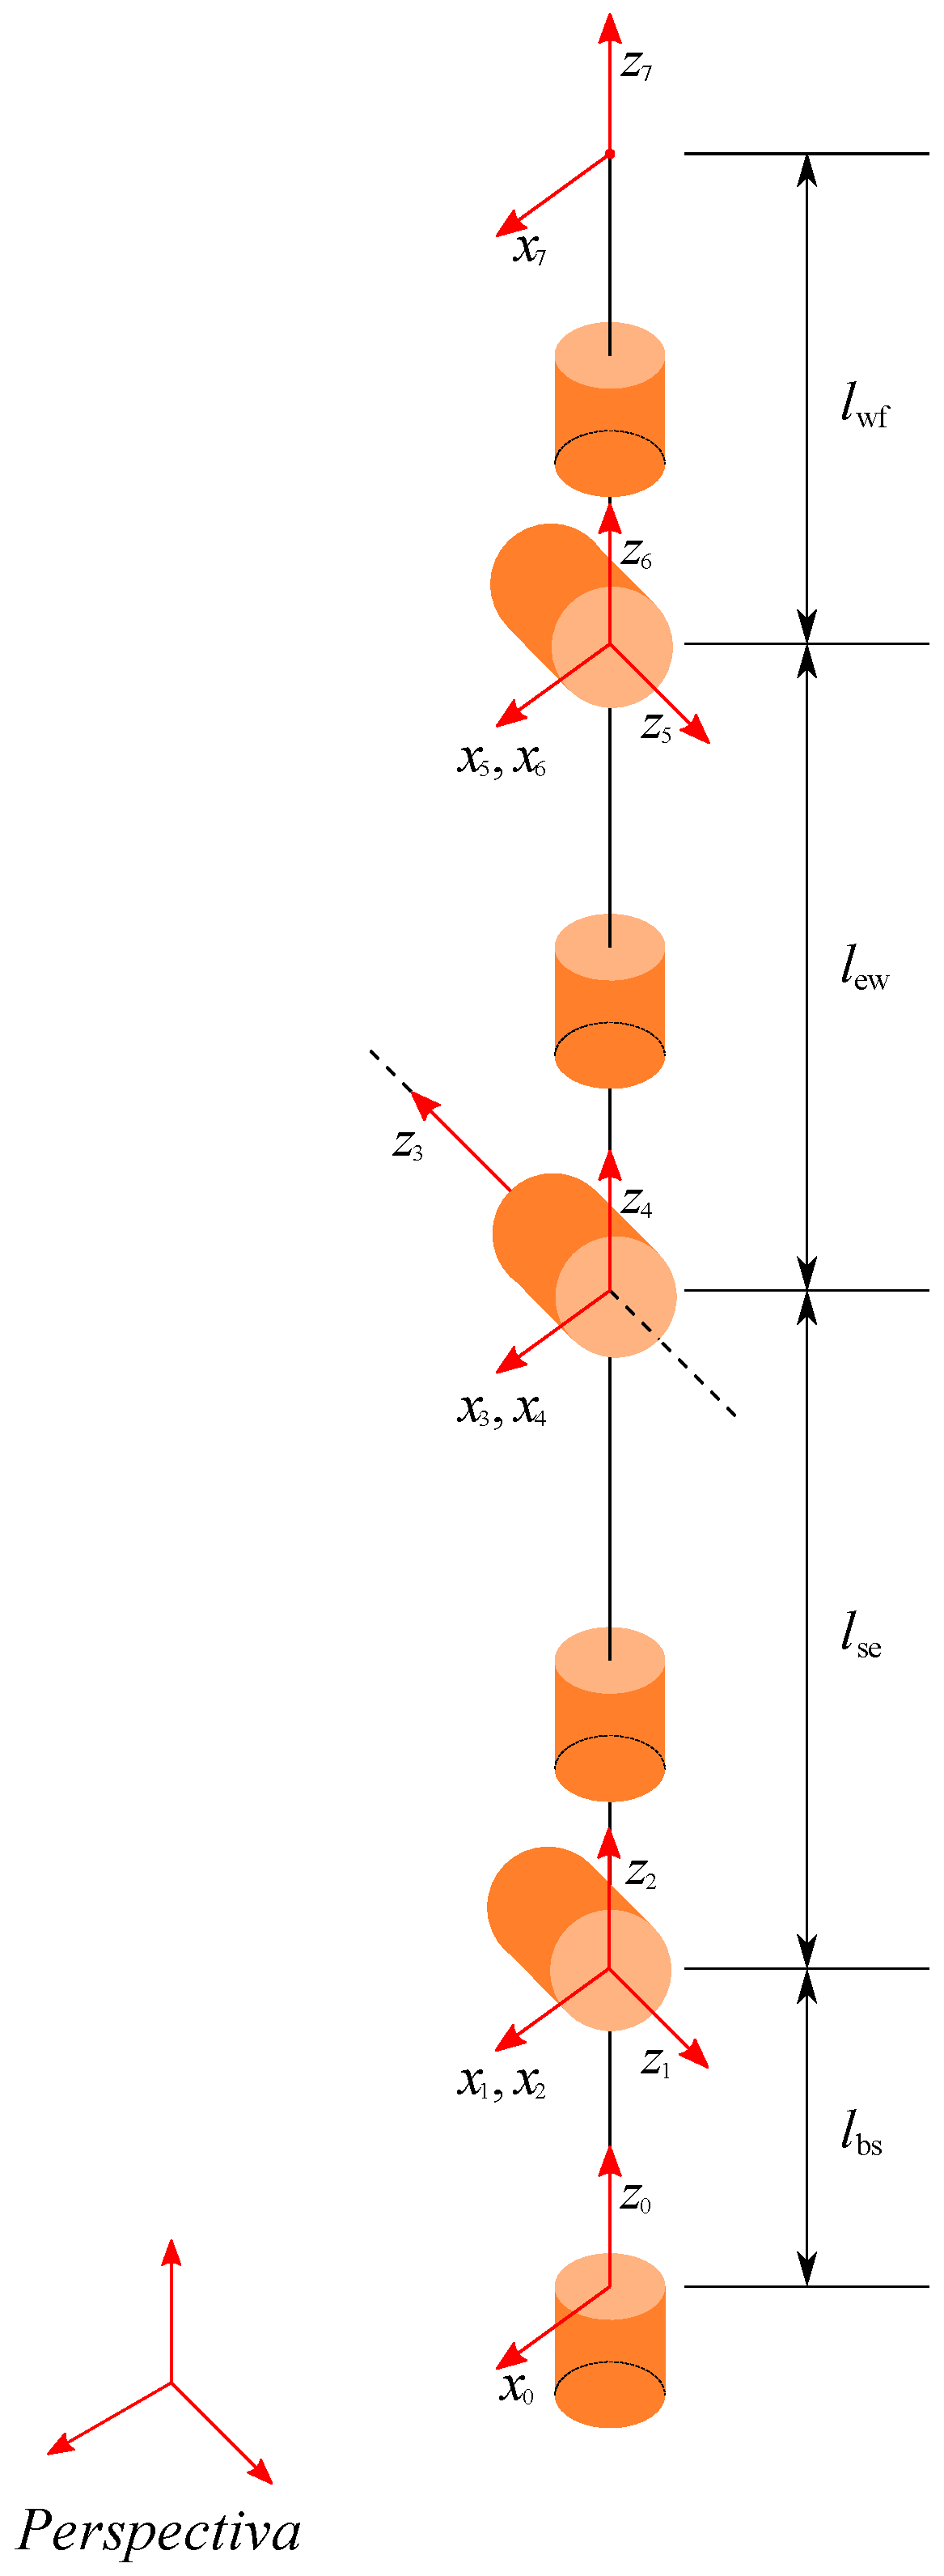
\includegraphics[width=3.5cm]{Imagem/validacao_home.eps}
    \caption{Diagrama esquemático da posição home}
    \label{diagramahome}
\end{figure}

Já para a matriz $T_\mathrm{escolhida}$, tem-se rotação de $-\ang{90}$ em $\theta_4$, o que distribui as translações nos eixos $z_0$, com valor de 780 mm representando a soma dos links $bs$ e $se$ ou do \textit{frame} zero ao quatro, e o restante da extensão do robô, 490 mm, fica direcionado paralelamente ao eixo $x_0$.

Após a curvatura de $-\ang{90}$ em $\theta_4$, tem-se a rotação do link 5 que faz com que o restante do braço do robô rotacione. O \textit{frame} final se dá portanto pelo resultado de uma composição de duas rotações e das translações relacionadas acima relação ao \textit{frame} zero.

O diagrama de arames mostrado na FIG. \ref{fig:condicaoescolhida} mostra os passos tomados para a avaliação desta nova pose. Em (a) o frame 4 é rotacionado em $-\ang{90}$; em (b) é feita a composição total do robô para tal rotação. Para (c) é mostrada a rotação do eixo 5 devido a rotação em $\theta_5$ e (d) é mostrado a configuração final do robô.

\begin{figure}[h]
    \centering
    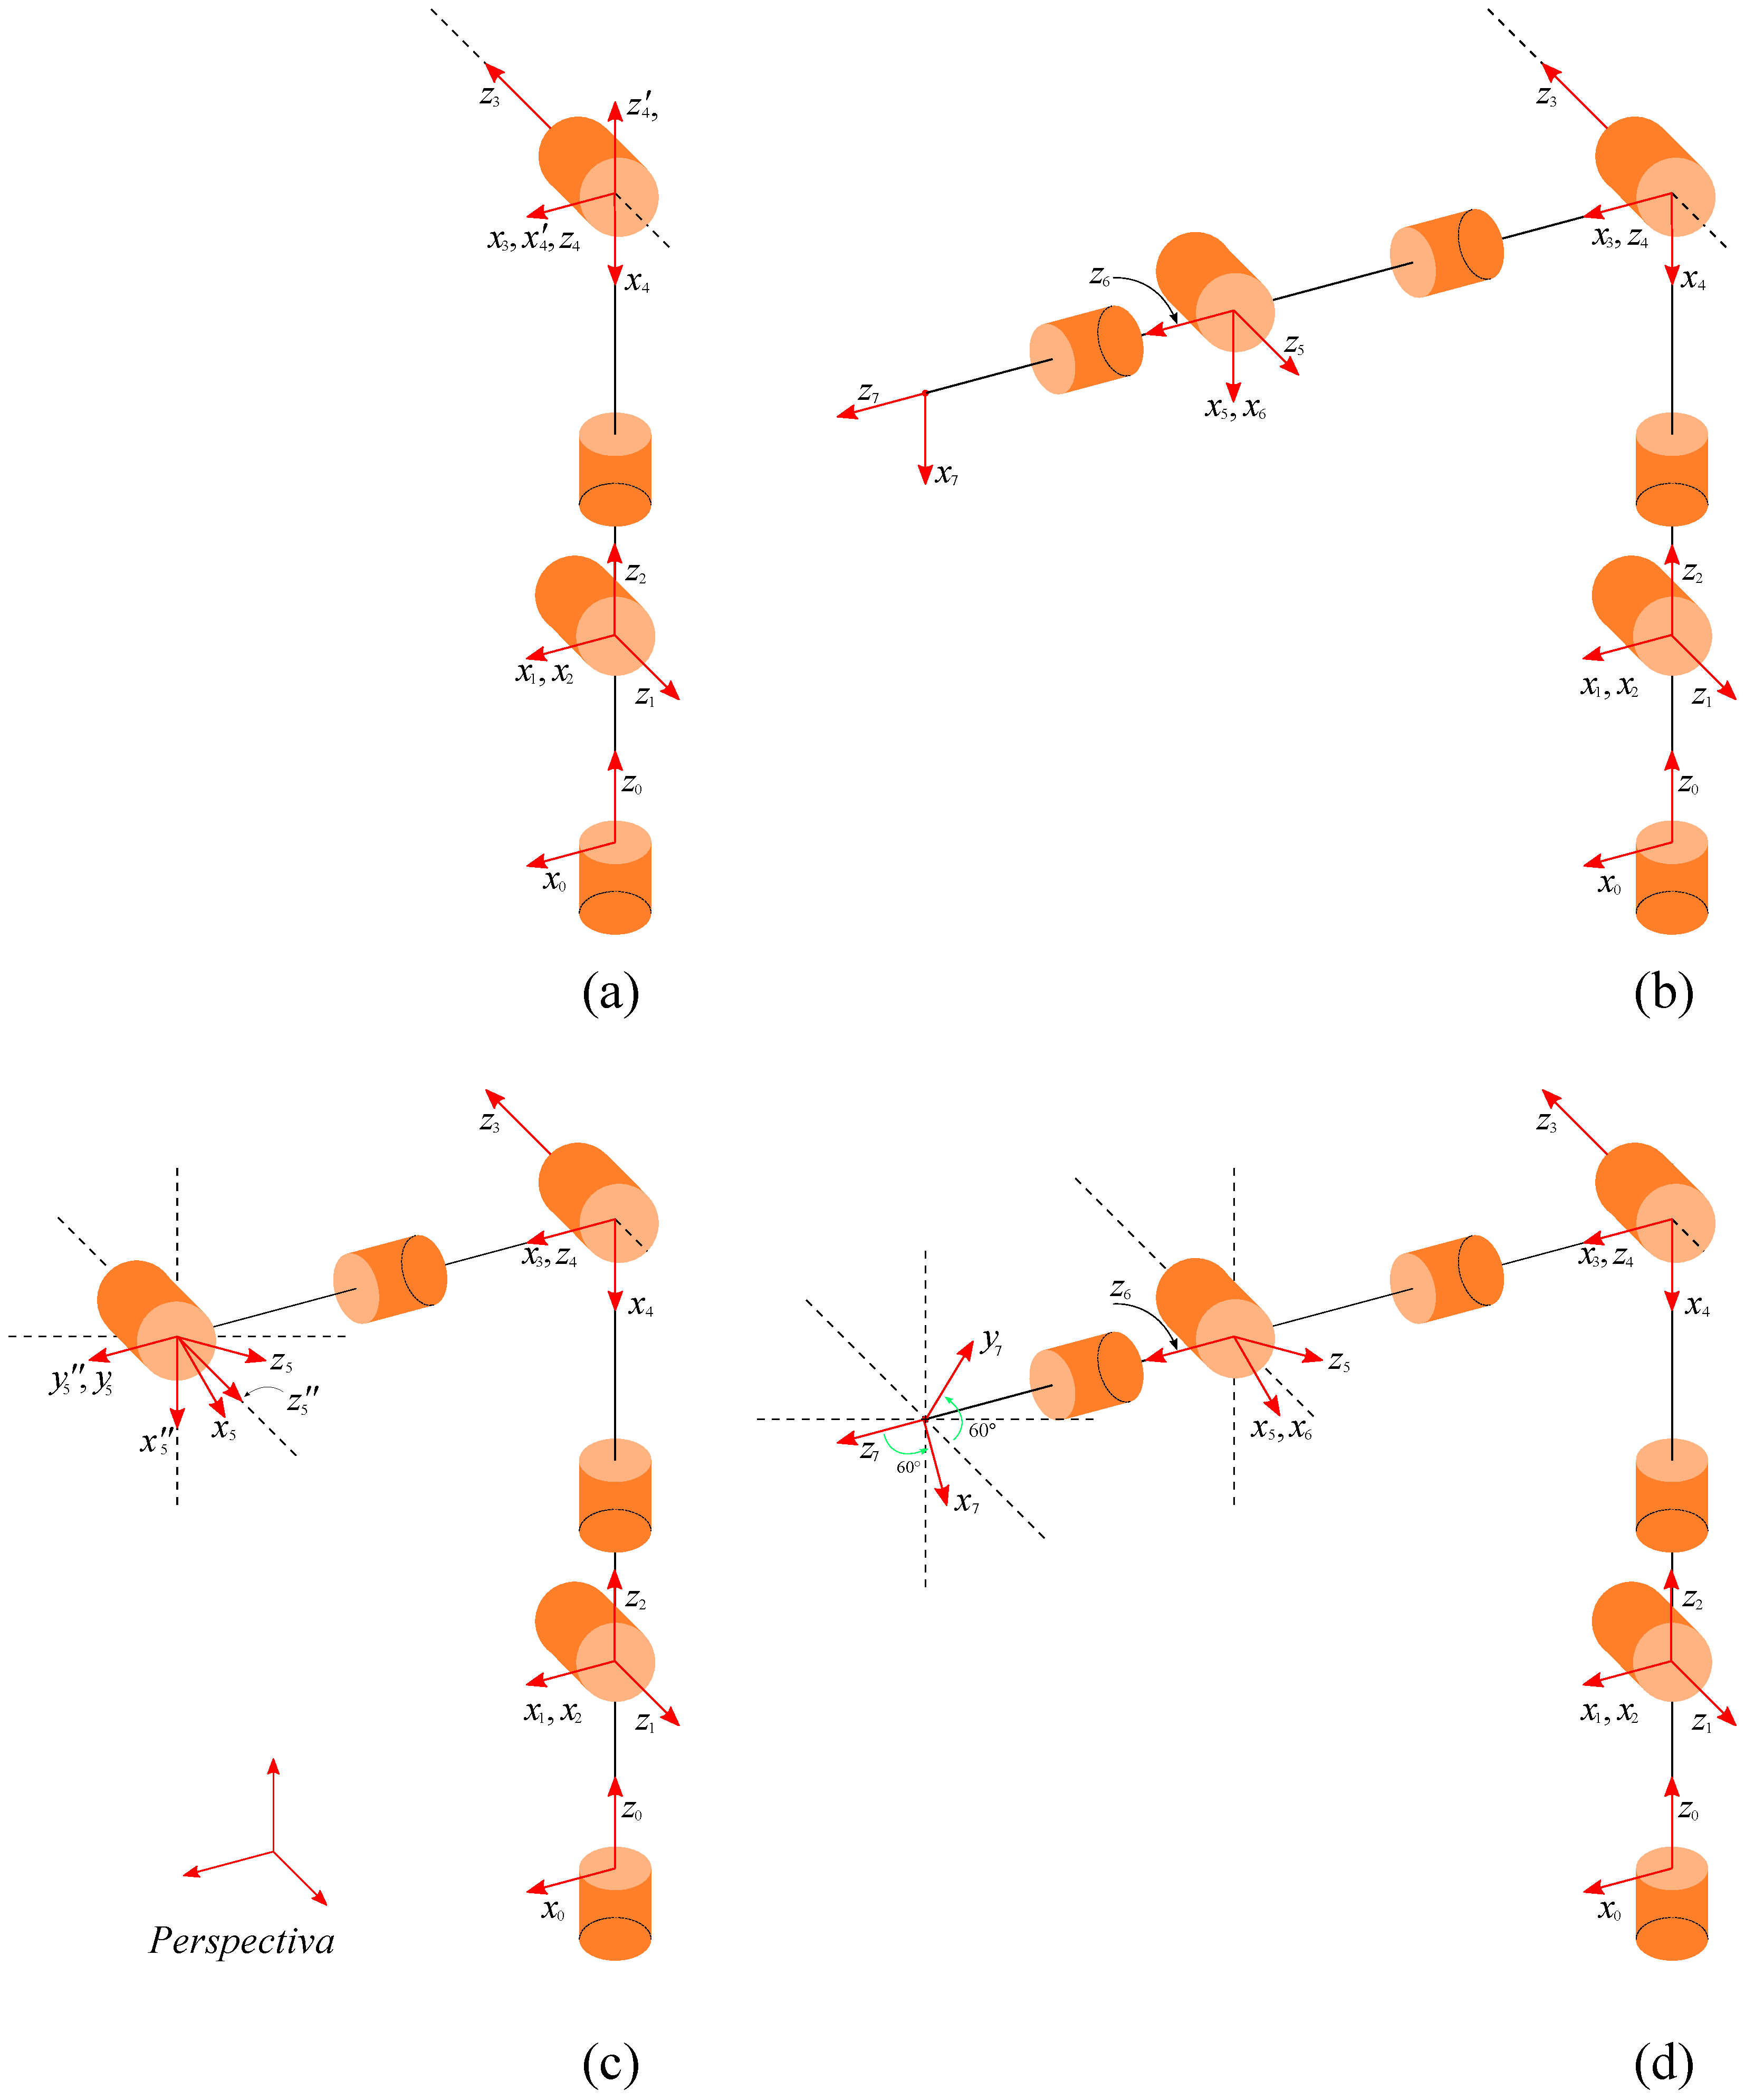
\includegraphics[width=8cm]{Imagem/validacao.eps}
    \caption{Passo-a-passo da representação esquemática da posição escolhida}
    \label{fig:condicaoescolhida}
\end{figure}

Note que a rotação do \textit{end-effector} pode ser analisando resolvendo
\begin{equation}
    R_7^0 = \Big[ x_7^0 \:\big|\: y_7^0 \:\big|\: z_7^0 \Big] = \left[\begin{array}{ccccc}
        x_7 \cdot x_0 && y_7 \cdot x_0 && z_7 \cdot x_0 \\
        x_7 \cdot y_0 && y_7 \cdot y_0 && z_7 \cdot y_0 \\
        x_7 \cdot z_0 && y_7 \cdot z_0 && z_7 \cdot z_0
    \end{array}\right]
    \label{eq:matrizR_generica}
\end{equation}

Na FIG. \ref{fig:zoom_pose_escolhido} nota-se inicialmente que $z_7 \cdot x_0 = 1$ então $x_7 \cdot x_0 = 0$, $y_7 \cdot x_0 = 0$, $z_7 \cdot y_0 = 0$ e $z_7 \cdot z_0 = 0$, visto que a matriz de rotação é ortonormal.
\begin{figure}[h]
    \centering
    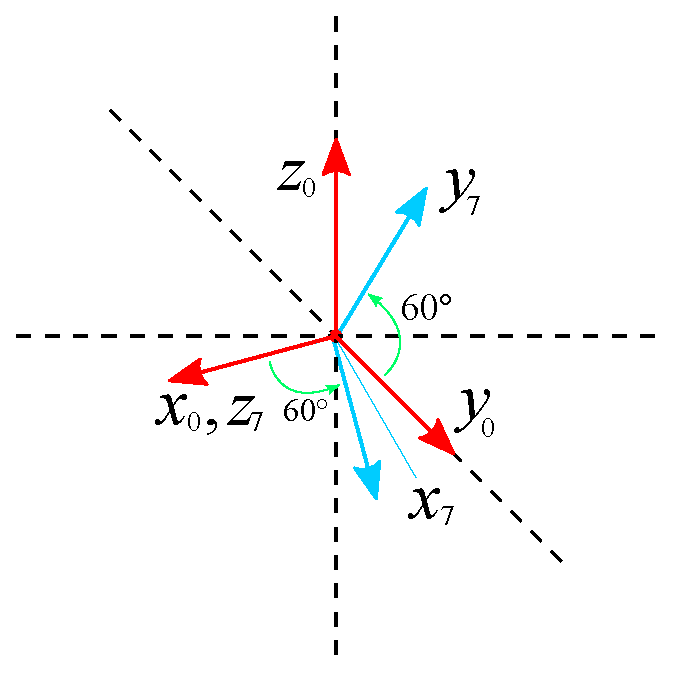
\includegraphics[width=5cm]{Imagem/zoom_pos-escolhida.eps}
    \caption{Orientação do \textit{end-effector}}
    \label{fig:zoom_pose_escolhido}
\end{figure}

Fazendo a projeção de $x_7$ em $y_0$ segue $\sen \ang{60} = \sqrt{3}/2$. Para $x_7$ em $z_0$, temos $-\cos \ang{60}$. Ainda, repetindo o processo para $y_7$, chega-se a $y_7 \cdot y_0 = \cos \ang{60}$ e $y_7 \cdot z_0 = \sen \ang{60}$. Portanto, a matriz que representa a orientação do \textit{frame} 7 é
\begin{equation}
    R_7^0 = \left[\begin{array}{rrrrr}
        0 && 0 && 1 \\
         \sqrt{3}/2 && 1/2 && 0 \\
        -1/2 && \sqrt{3}/2 && 0
    \end{array}\right]
    \label{eq:R_validacao}
\end{equation}

Comparando \eqref{eq:Tescolhido} com \eqref{eq:R_validacao}, verifica-se que a orientação da matriz de transformação é como se esperava. Destarte, o modelo cinemático do robô KUKA iiwa obtido foi validado.
